Durant notre première séance de laboratoire pour le cours de physique des télécommunications, nous avons dimensionné une antenne patch alimentée par une ligne microstrip à l'aide du logiciel FEKO. Pour cela nous avons procédé par étapes, partant d'un design simple et parfaitement symétrique auquel nous avons petit à petit ajouté ou modifié des éléments pour arriver à la version finale remplissant toutes les spécifications.

A la fin de la séance, nous avons obtenu une antenne dont les caractéristiques simulées étaient un coefficient de réflexion minimal de \SI{-27.43}{\deci\bel} à la fréquence de \SI{2.398}{\giga\hertz}\footnote{Le cahier des charges nous imposait un coefficient de réflexion de \SI{-6}{\deci\bel} à la fréquence d'utilisation de l'antenne, c'est-à-dire \SI{2.4}{\giga\hertz}}, et un gain maximal de \num{2.54}.

Cette antenne sera ensuite testée expérimentalement lors de la troisième séance. Dans ce chapitre, nous allons détailler les différentes étapes qui nous ont amenés au dimensionnement final de notre antenne.

\subsection{Antenne sur un diélectrique infini}
Pour commencer, nous avons simplement simulé un patch rectangulaire en matériau conducteur parfait posé sur une plaque infinie en matériau diélectrique de même permittivité électrique que le PCB utilisé en pratique pour fabriquer notre antenne, mais considéré dans un premier temps sans perte. Les dimensions du patch ont été calculées à partir de la fréquence d'utilisation souhaitée ainsi que de l'épaisseur et de la permittivité du diélectrique utilisé, en utilisant les relations fournies dans l'énoncé. La figure \ref{fig:rayonnement_11} nous donne la directivité ainsi que le gain de l'antenne pour des valeurs de $\phi$ de \SI{0}{\degree} et \SI{90}{\degree}.
\begin{figure}[htbp]
  \centering
  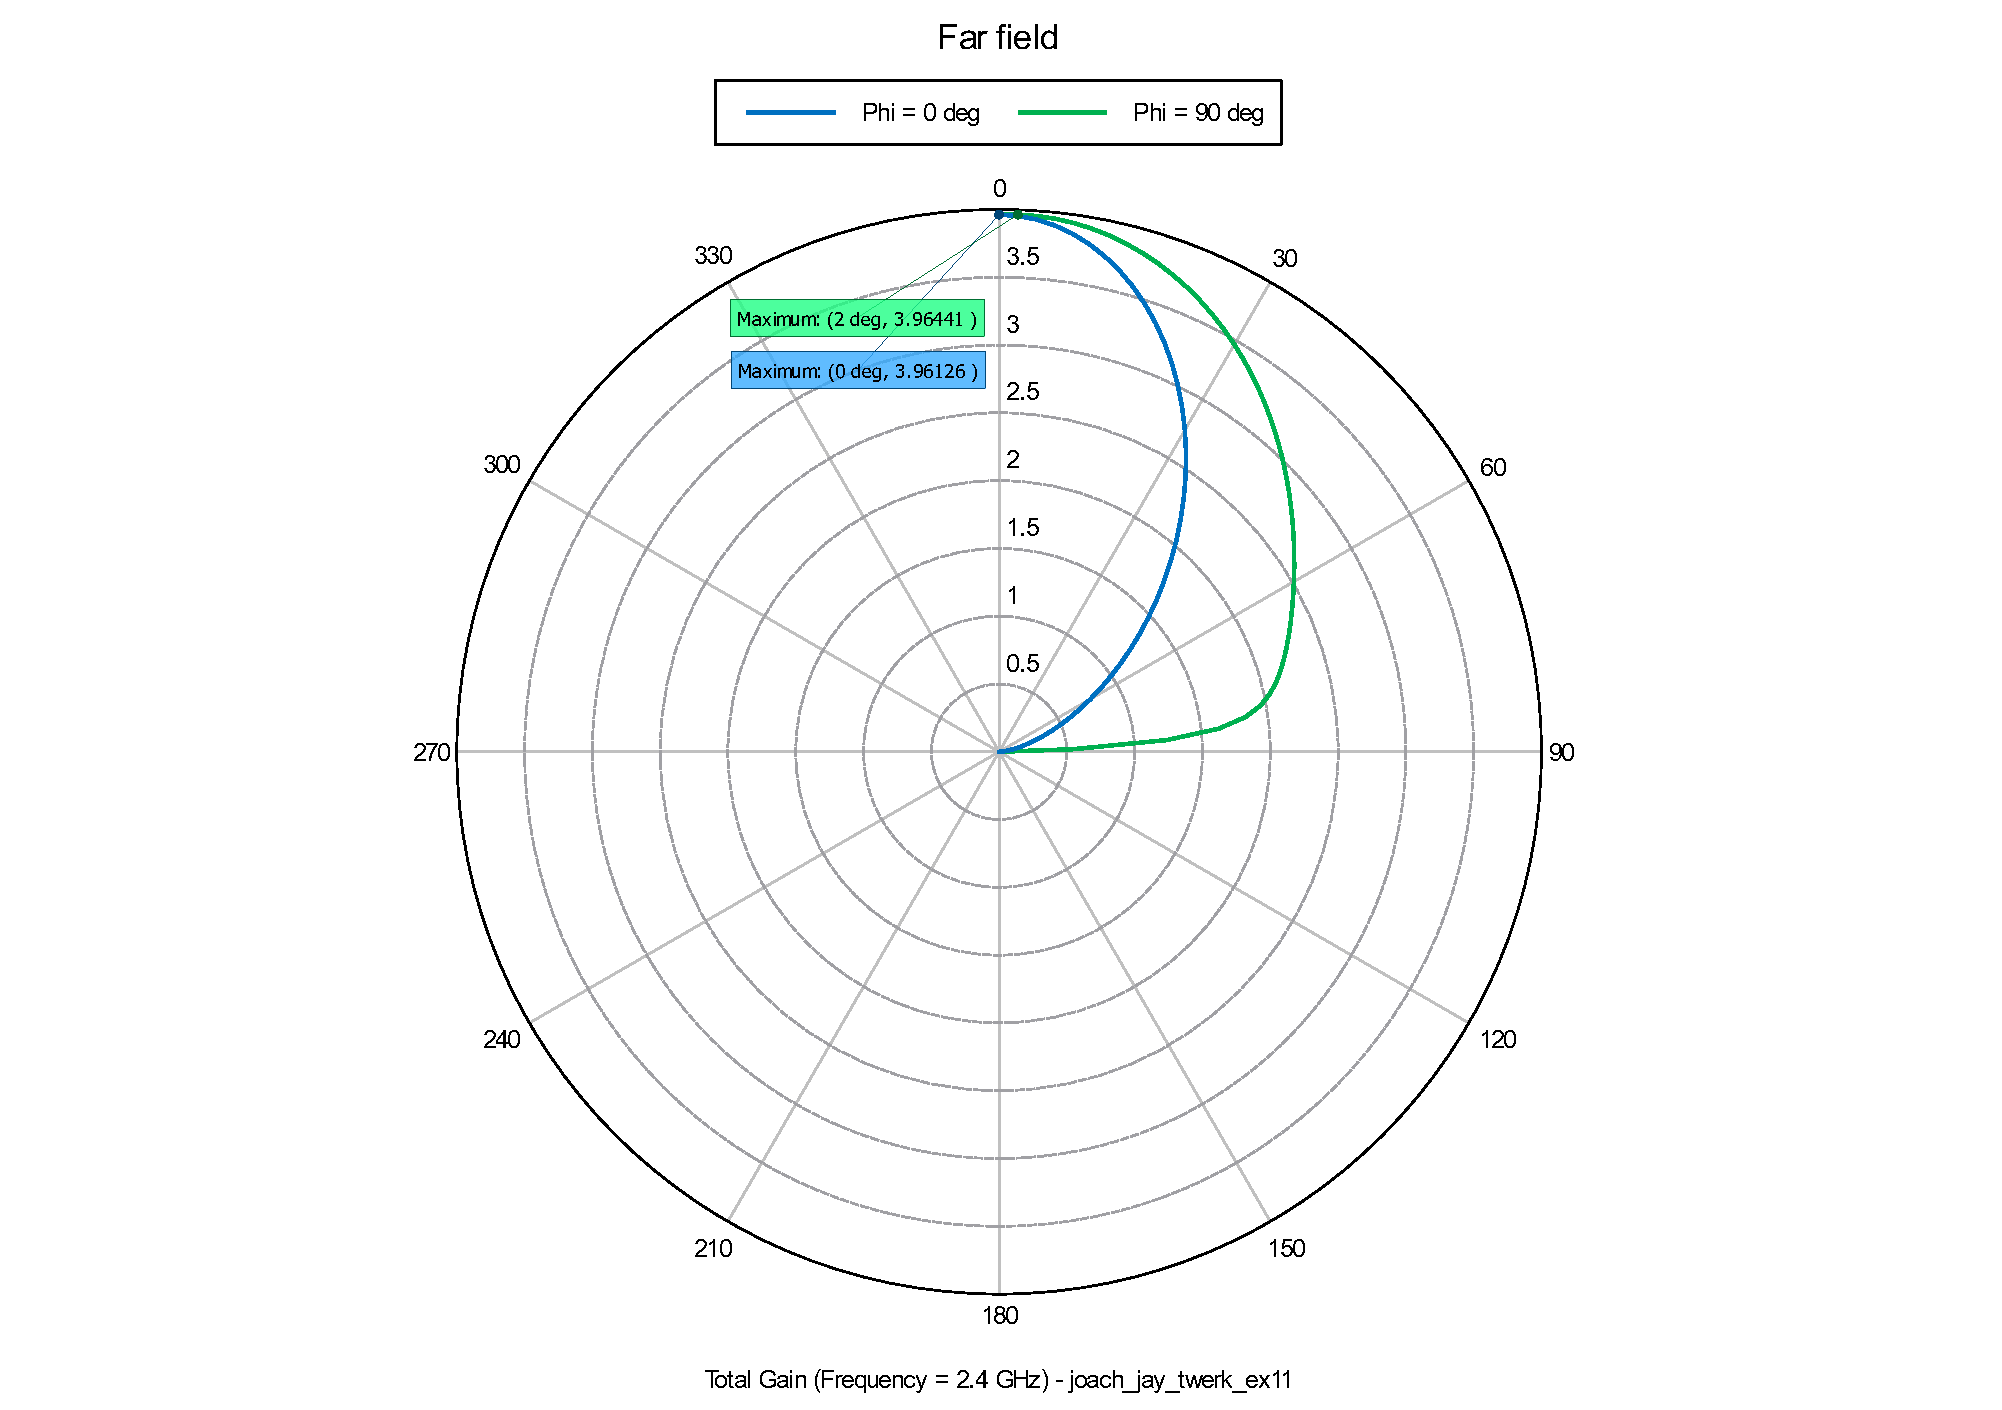
\includegraphics[width=\textwidth]{rayonnement11_annotation.pdf}
  \caption{Diagramme de rayonnement du gain \label{fig:rayonnement_11}}
\end{figure}
La directivité et le gain ont des valeurs égales car, pour l'instant, nous avons fait nos simulations sans pertes: $\eta = 1$

Nous nous sommes aussi intéressés au coefficient de réflexion de l'antenne, qui dépend fortement de la fréquence d'excitation.
\begin{figure}[htbp]
  \centering
  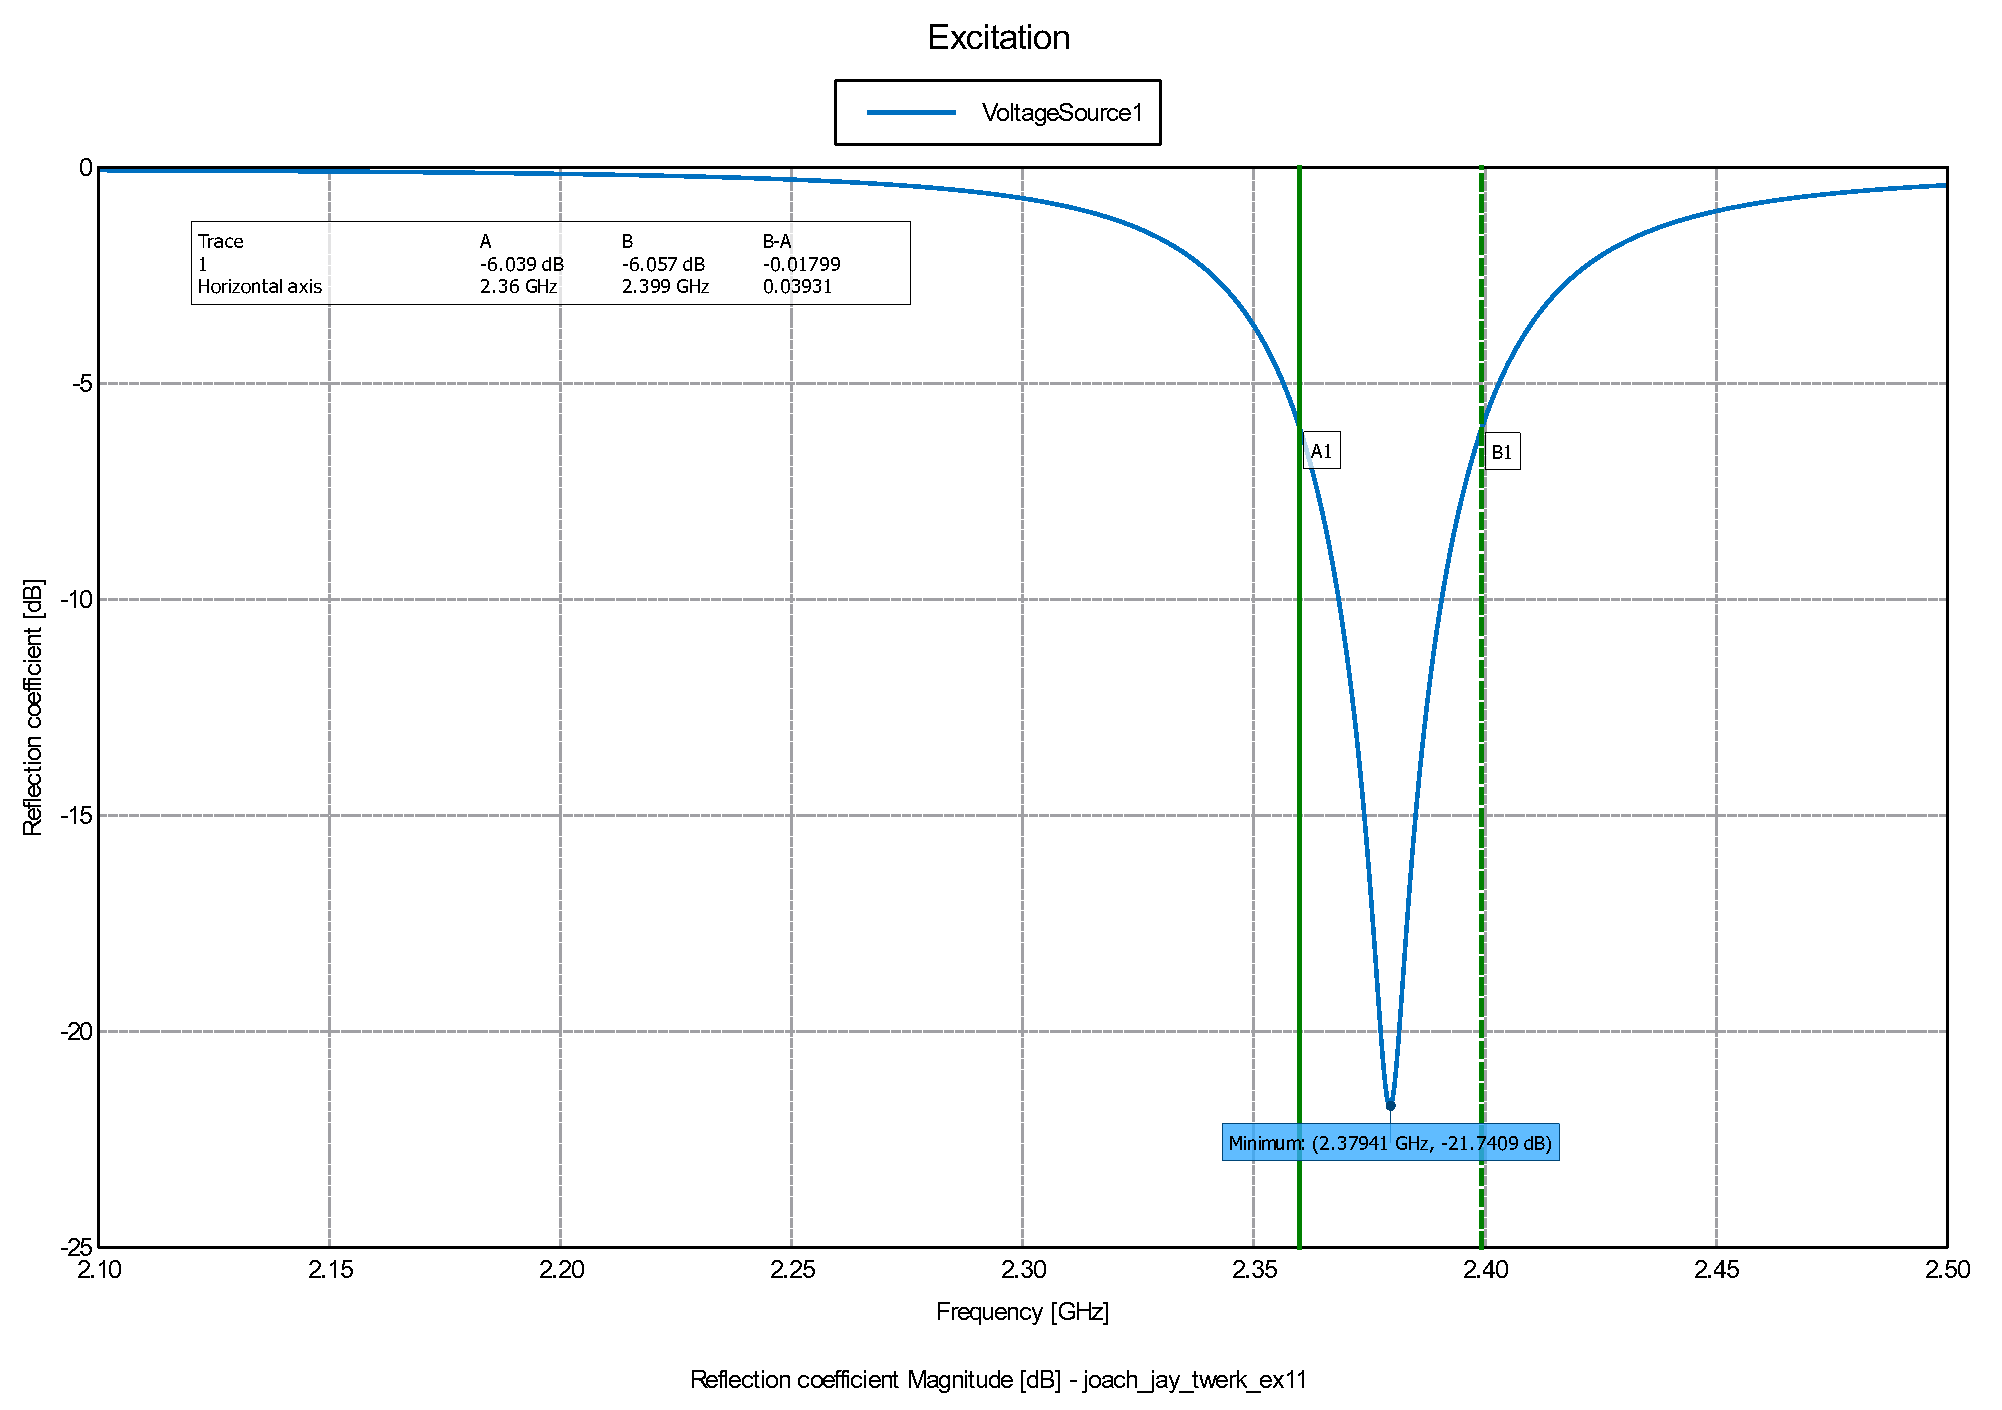
\includegraphics[width=\textwidth]{reflection11_annotation.pdf}
  \caption{Coefficient de réflexion en fonction de la fréquence [généré avec PostFeko]\label{fig:reflection11_}}
\end{figure}
La figure \ref{fig:reflection11_} nous montre que la résonance de l'antenne se situe à \SI{2.38}{\giga\hertz} et qu'à cette fréquence le coefficient de réflexion vaut \SI{-21.8}{\deci\bel}. A la fréquence d'intérêt de \SI{2.4}{\giga\hertz}, ce coefficient vaut \SI{-6}{\deci\bel}. Il est aussi intéressant de noter la largeur de la bande passante\footnote{Définie ici comme l'intervalle de fréquence ou $\Gamma_L < \SI{-6}{\deci\bel}$} qui vaut dans ce cas près de \SI{0.04}{\giga\hertz}.

A partir de ces mesures, nous pouvons calculer le pourcentage de puissance délivrée à l'antenne à la fois à la fréquence de résonance et à \SI{2.4}{\giga\hertz}. Ce pourcentage est obtenu par la relation \ref{eqn:puissance délivrée}, qui nous donne une valeur de \SI{99.3}{\percent} à la fréquence de résonance et \SI{75.2}{\percent} à \SI{2.4}{\giga\hertz}.
\begin{equation}
\frac{P_L}{P_{in}} = 1-{\Gamma_L}^2
\label{eqn:puissance délivrée}
\end{equation}

%Note pour jojol: coeff de réflection c'est gamma majuscule, aka \Gamma_L (L pour load).
%Merci d'utiliser \SI! c'est vachement cool!
%Je me suis planté, la proportion absorbée c'est 1-(gamma)². Je m'occupe (ou me suis occupé) de corriger dans ce qui est déjà fait.
%Largeur des figures = \textwidth? Sinon je trouve qu'elles ne sont pas super lisibles
%NOTE POUR TWERKYTWERK : pour la largeur des figures je me suis 100pourcent inspiré des labos de thermo, je te laisse modifier la mise en forme à ta guise, je touche pas grand chose à ça

\subsection{Antenne sur un diélectrique fini}
Le pas suivant vers une antenne patch réelle consiste à remplacer le substrat infini par un carré de coté \SI{50}{\milli\meter}, c'est-à-dire la dimension du PCB de notre antenne. Ci-dessous, nous détaillons les changements dû à cette modification sur les différents paramètres déjà étudiés plus haut.

Premièrement, comme nous pouvons le voir sur la figure \ref{fig:reflection12_annotation},
\begin{figure}[htbp]
\centering
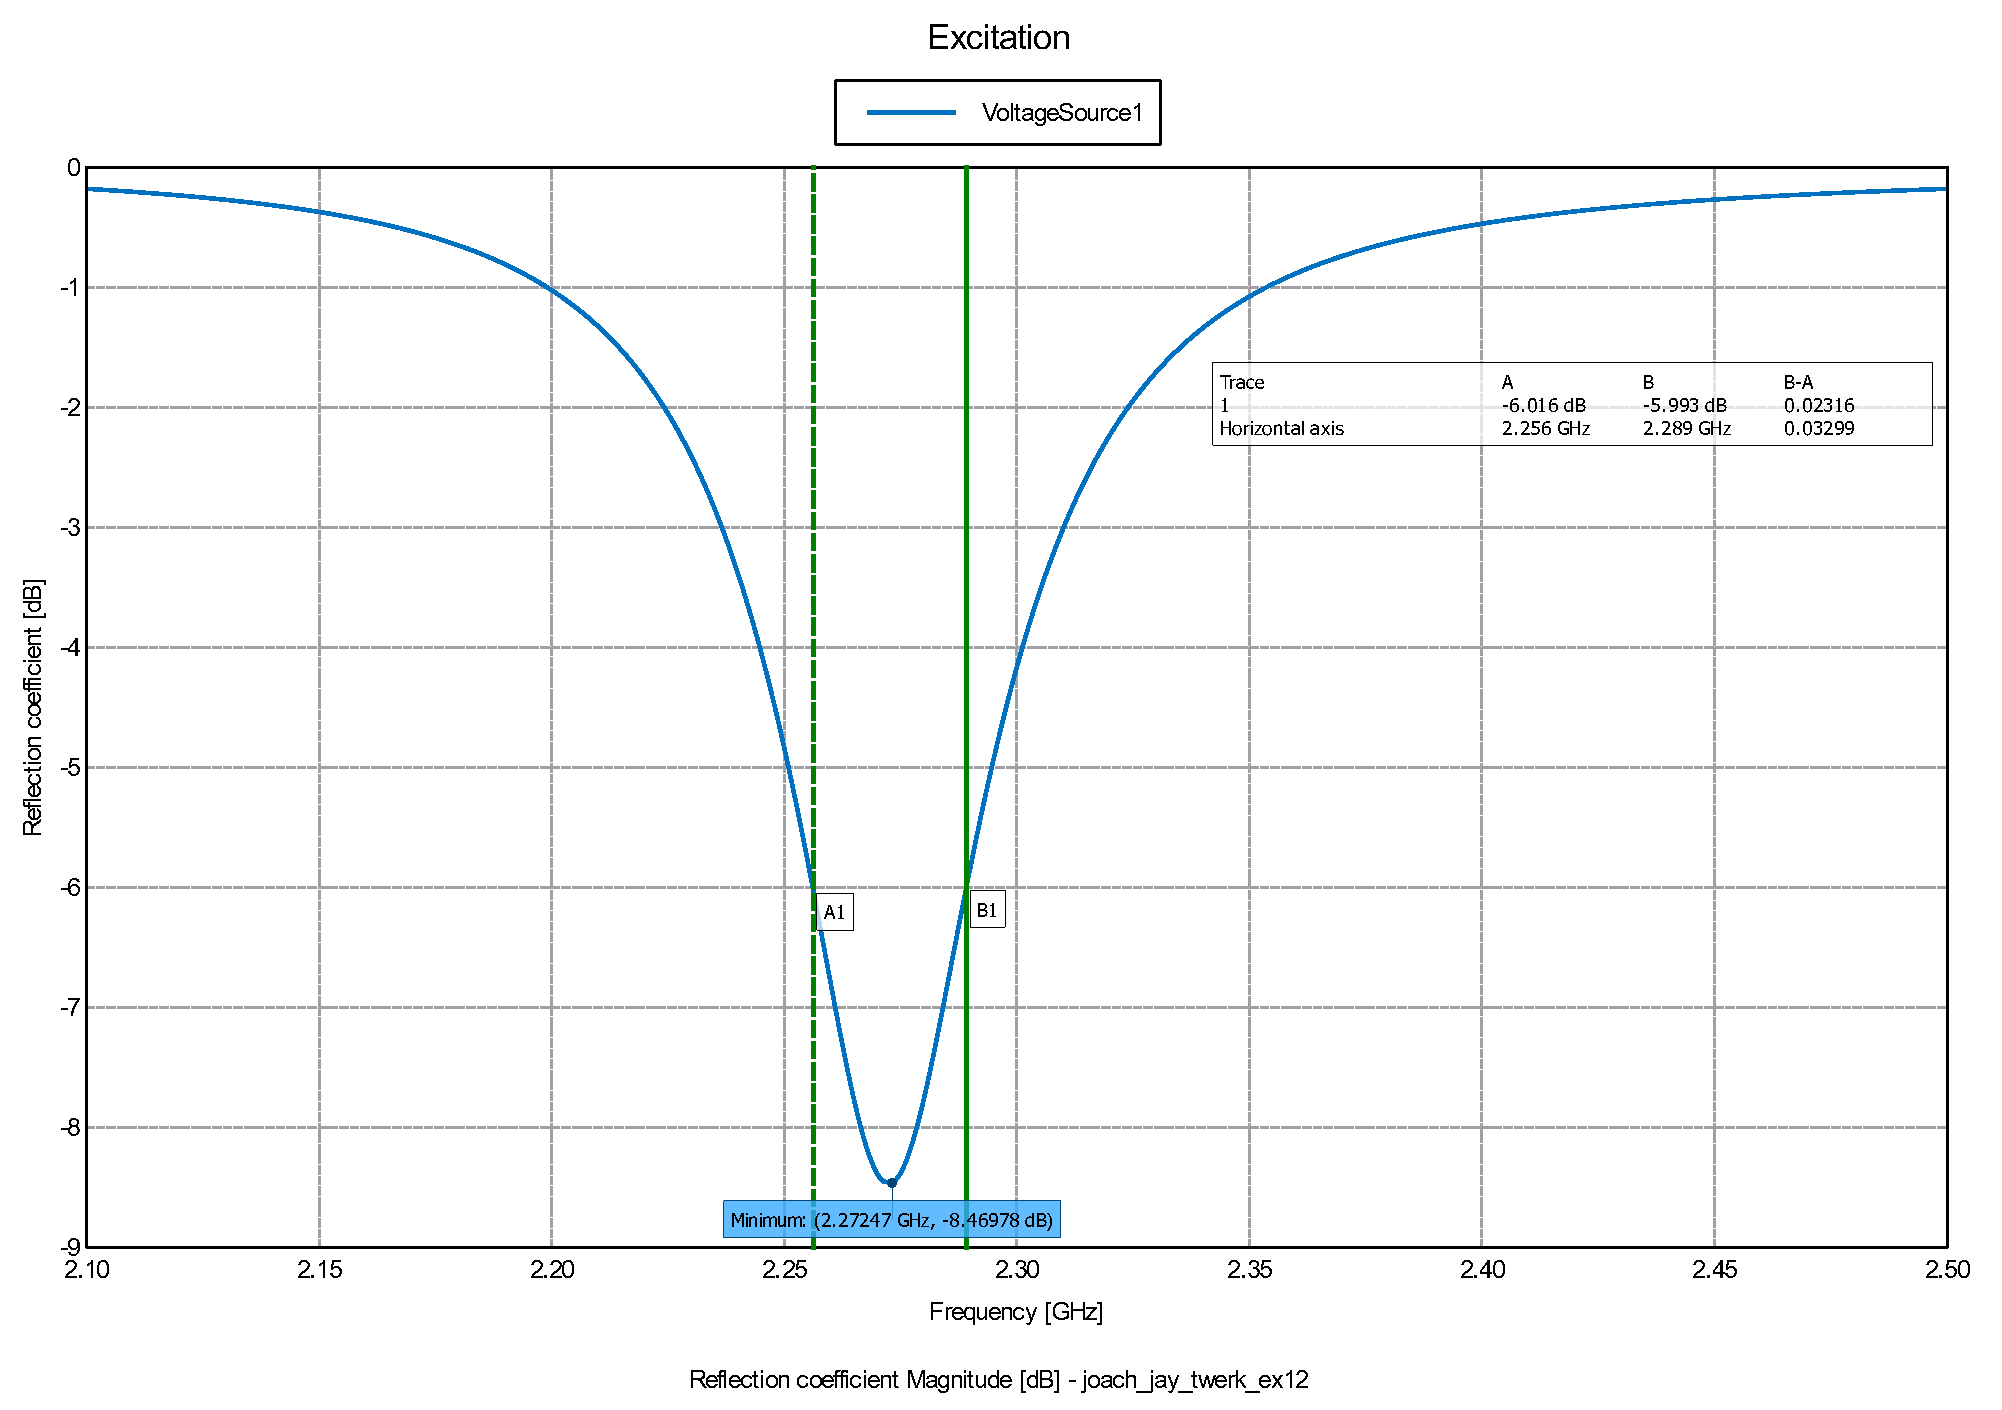
\includegraphics[width=\textwidth]{reflection12_annotation.pdf}
\caption{Coefficient de réflexion en fonction de la fréquence\label{fig:reflection12_annotation}}
\end{figure}
la fréquence de résonance s'est déplacée à \SI{2.27}{\giga\hertz} mais le coefficient de réflexion à surtout fortement augmenté pour prendre la valeur de \SI{-8.47}{\deci\bel}. La bande passante s'est elle aussi dégradée et ne vaut plus que \SI{0.033}{\giga\hertz}.

A nouveau, il est intéressant d'étudier le diagramme de rayonnement du gain de l'antenne, donné à la figure \ref{fig:rayonnement12_annotation}, où l'on remarque que la directivité maximale et le gain maximal valent \SI{3.64}{},	 que ce soit pour $\phi = \SI{0}{\degree}$ ou $\SI{90}{\degree}$.
\begin{figure}
\centering
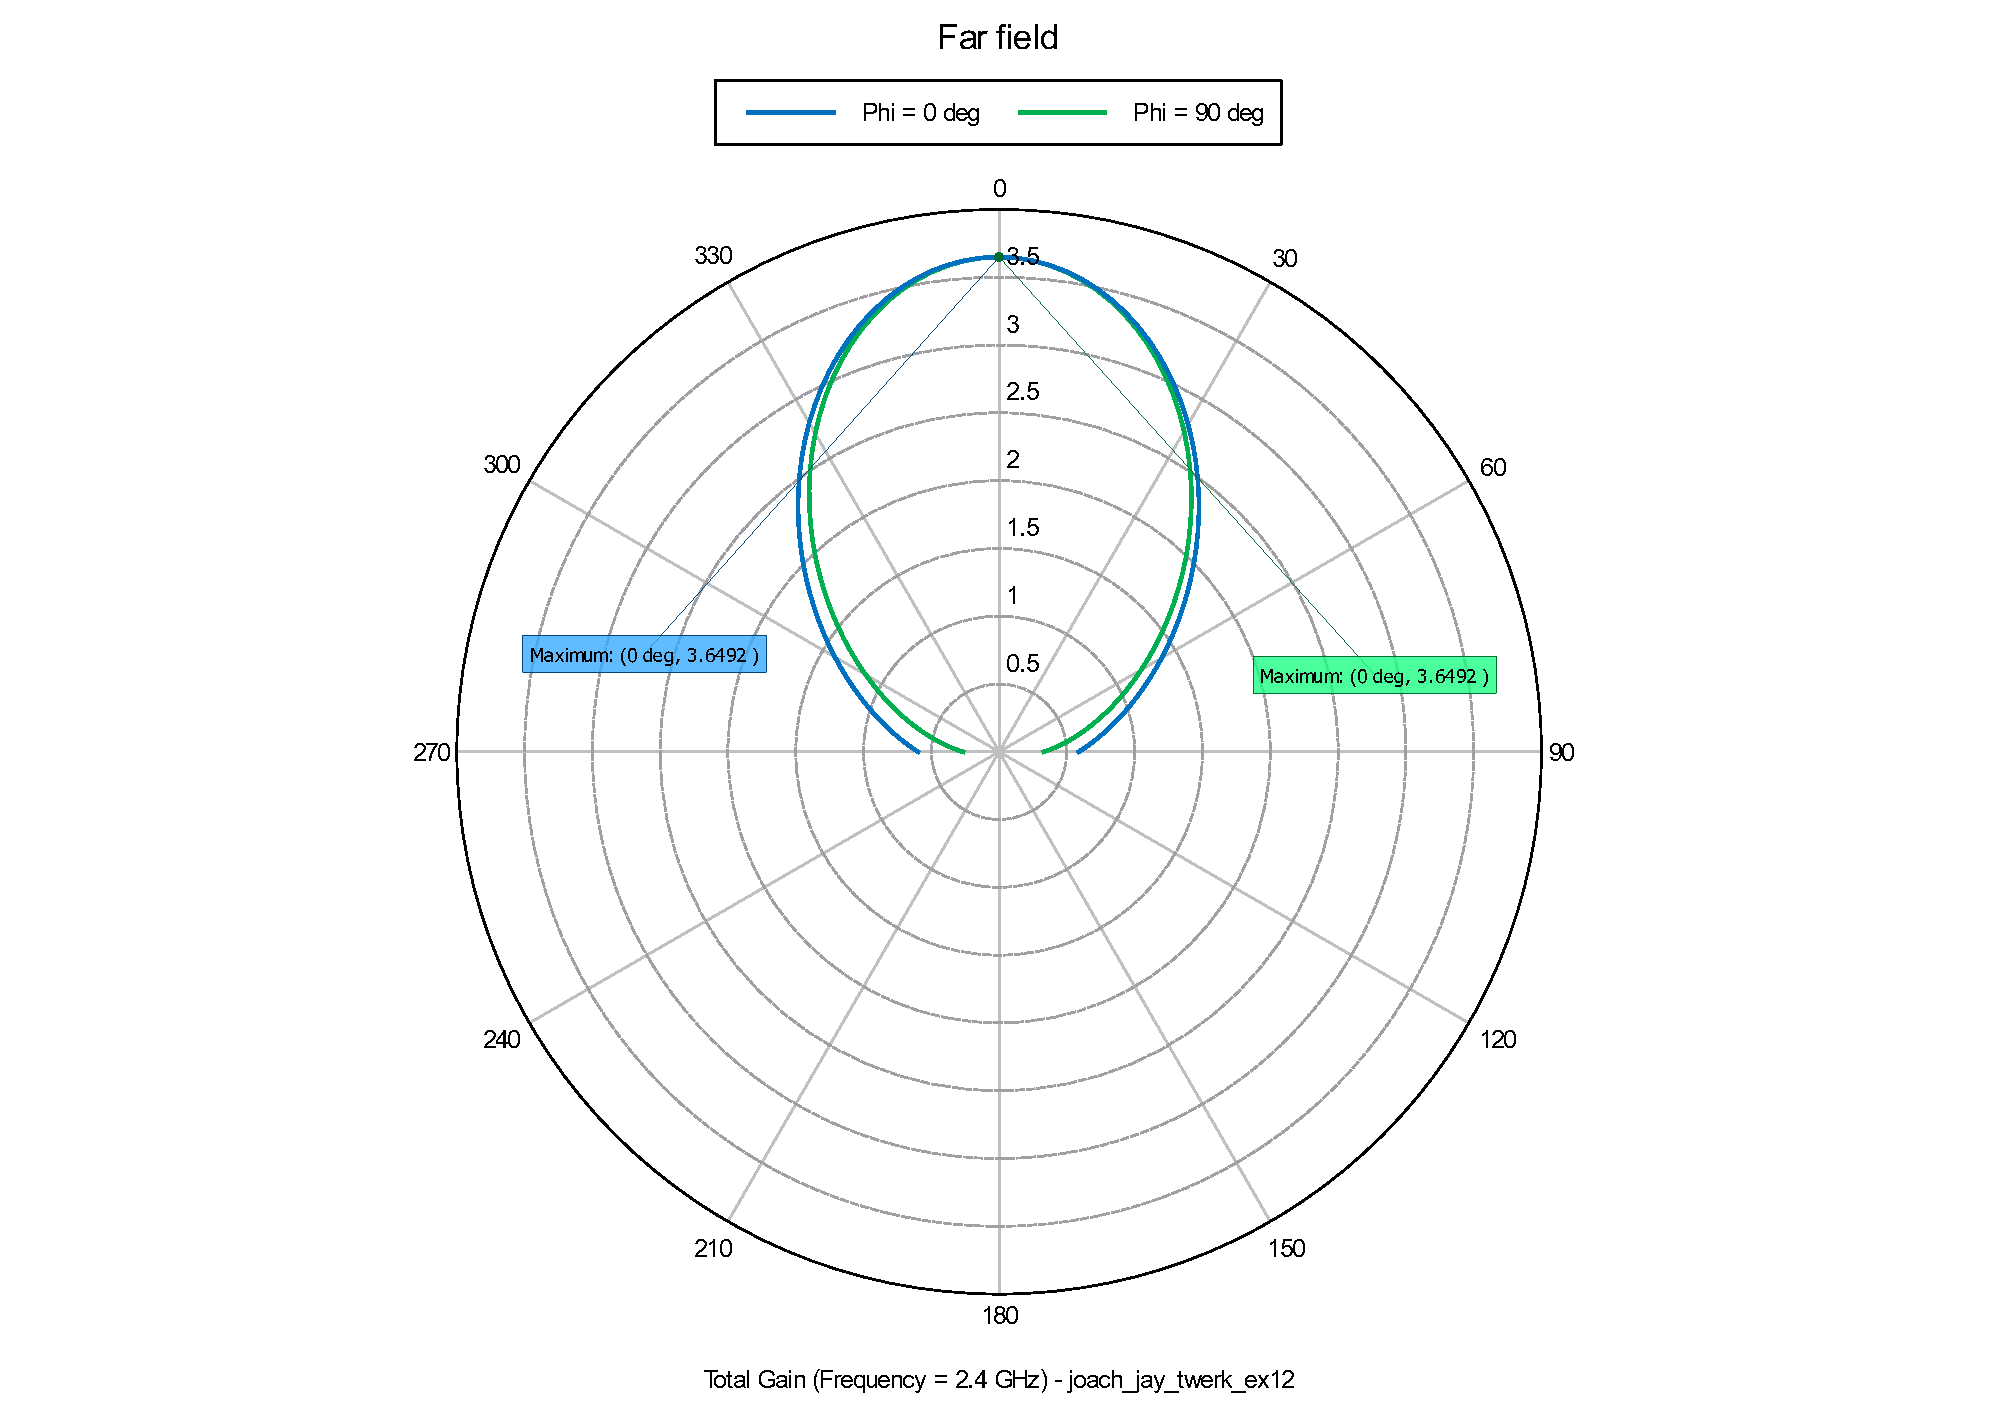
\includegraphics[width=\textwidth]{rayonnement12_annotation}
\caption{Diagramme de rayonnement de l'antenne sur diélectrique fini}
\label{fig:rayonnement12_annotation}
\end{figure}
Pour terminer, nous avons pris en compte les pertes dans le diélectrique en posant $\tan{\delta} = 0.01$. Le gain diminue alors à \num{2.64}, la directivité maximale vaut \SI{4.04}{} et le coefficient de réflexion vaut \SI{-6}{\deci\bel} à la fréquence de résonance, qui reste inchangée (figure \ref{fig:reflection122_annotation}).
\begin{figure}[htbp]
\centering
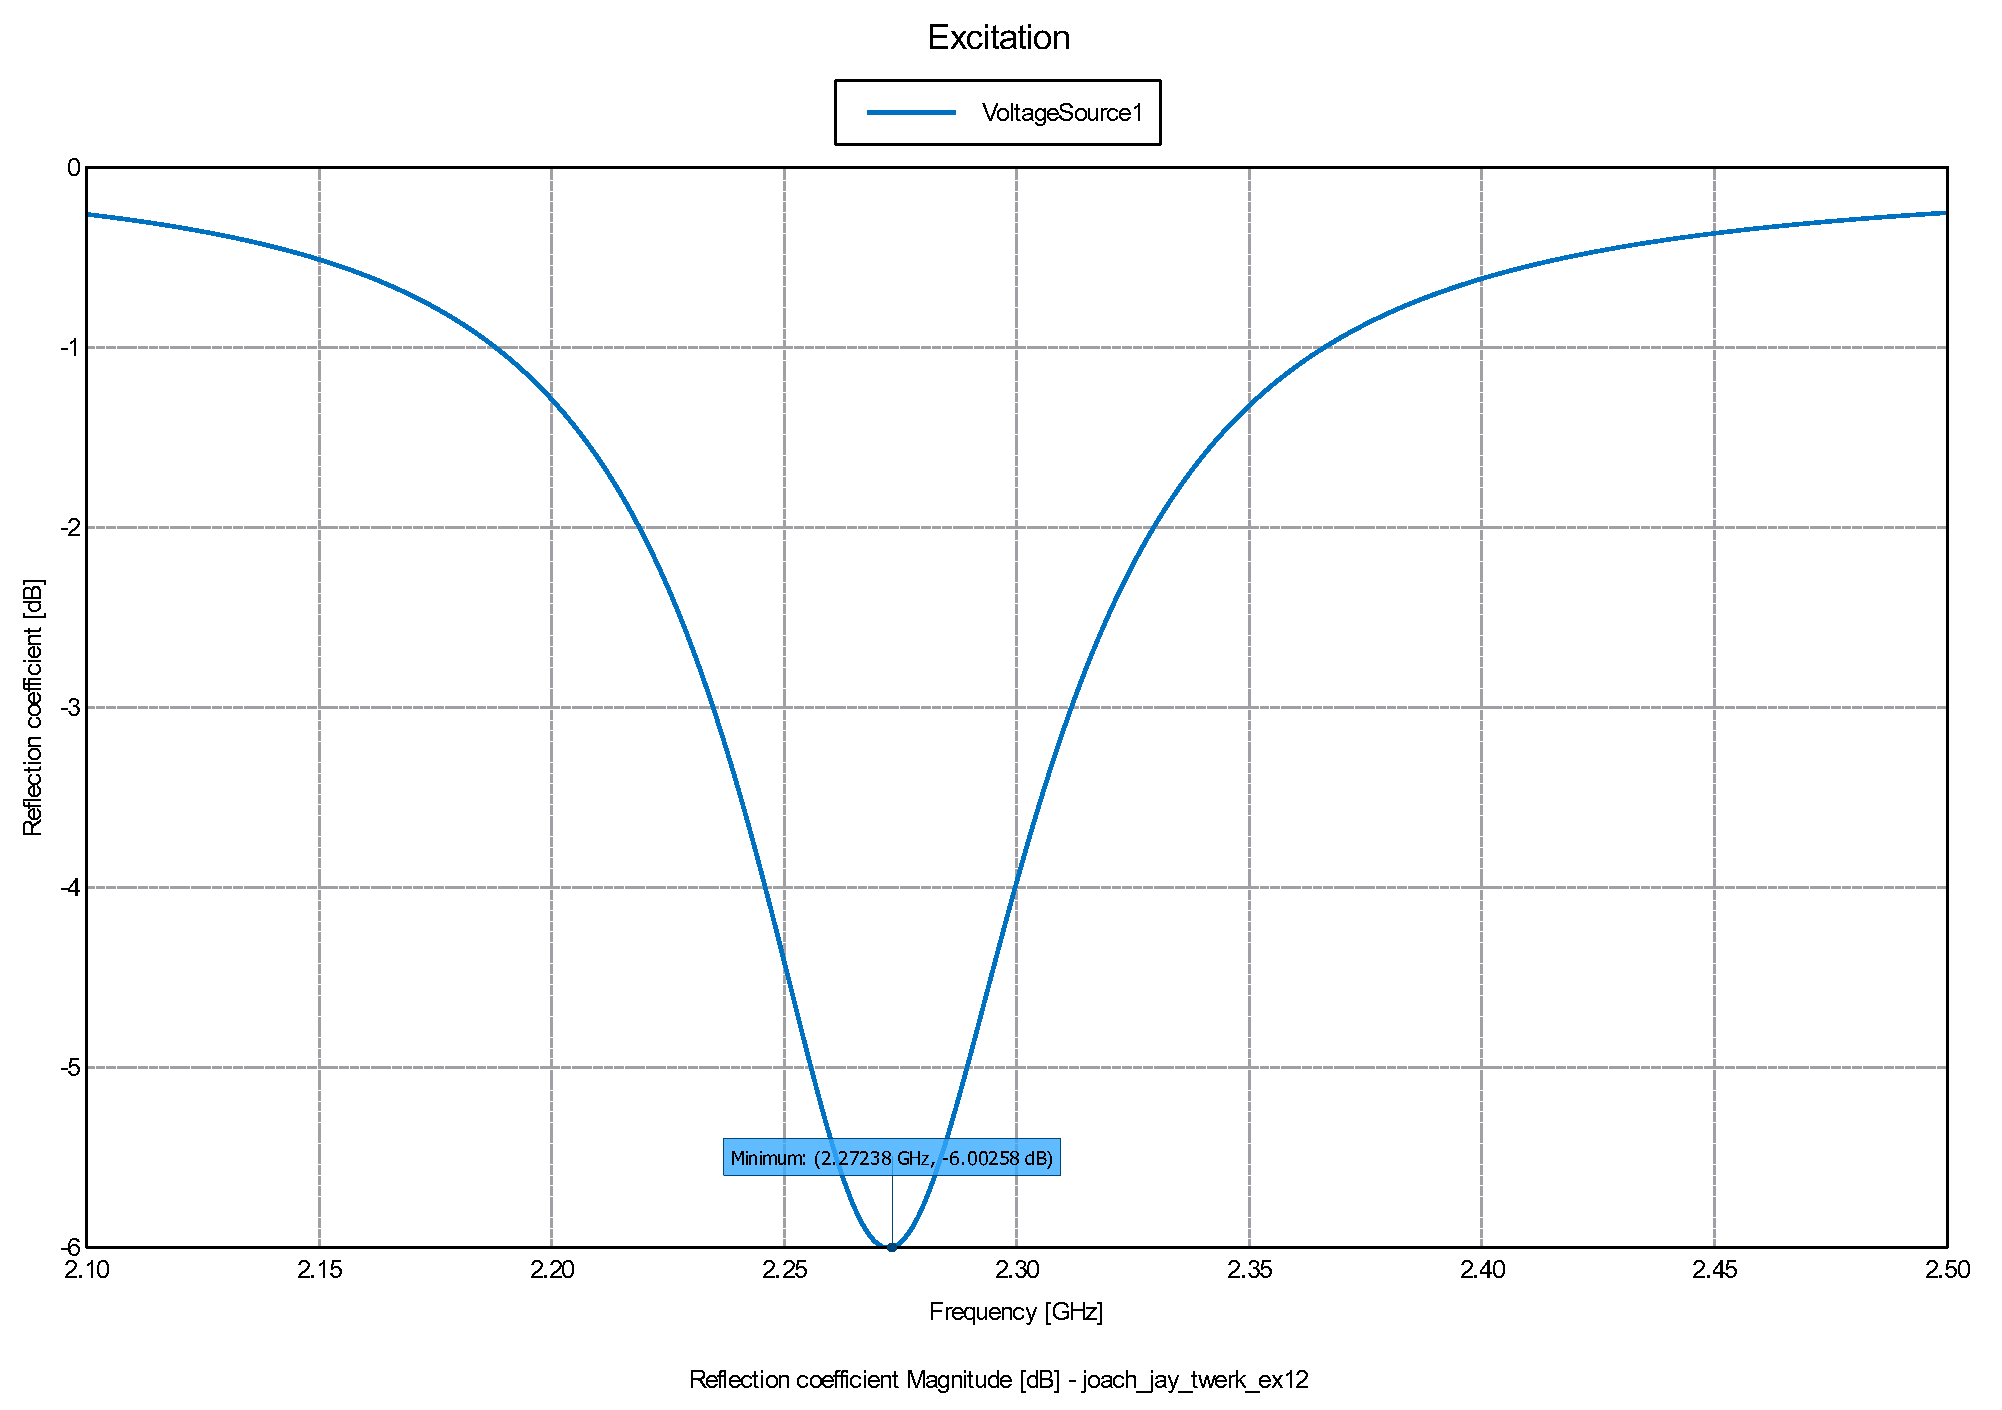
\includegraphics[width=\textwidth]{reflection122_annotation.pdf}
\caption{Coefficient de réflexion en fonction de la fréquence en tenant compte des pertes dans le diélectrique}
\label{fig:reflection122_annotation}
\end{figure}


\subsection{Antenne avec fente}
Comme l'indique le titre, l'étape suivante a été de ménager une fente dans le patch. La longueur de la fente est dimensionnée afin d'obtenir l'adaptation d'impédance à \SI{50}{\ohm} en utilisant les relations de l'énoncé qui relient $R_{in}(y=y_0)$ a $R_{in} (y= 0)$. La largeur est choisie assez grande pour éviter les que le champ émis par l'antenne ne se replie pas par la ligne microstrip. La spécification imposée était le coefficient de réflexion à la résonance qui devait être inférieur à \SI{-10}{\deci\bel}. Comme le montre la figure \ref{fig:reflection13_annotation}, notre choix de \SI{8}{\milli\meter} pour $y_0$ respecte cette consigne.
\begin{figure}[htbp]
\centering
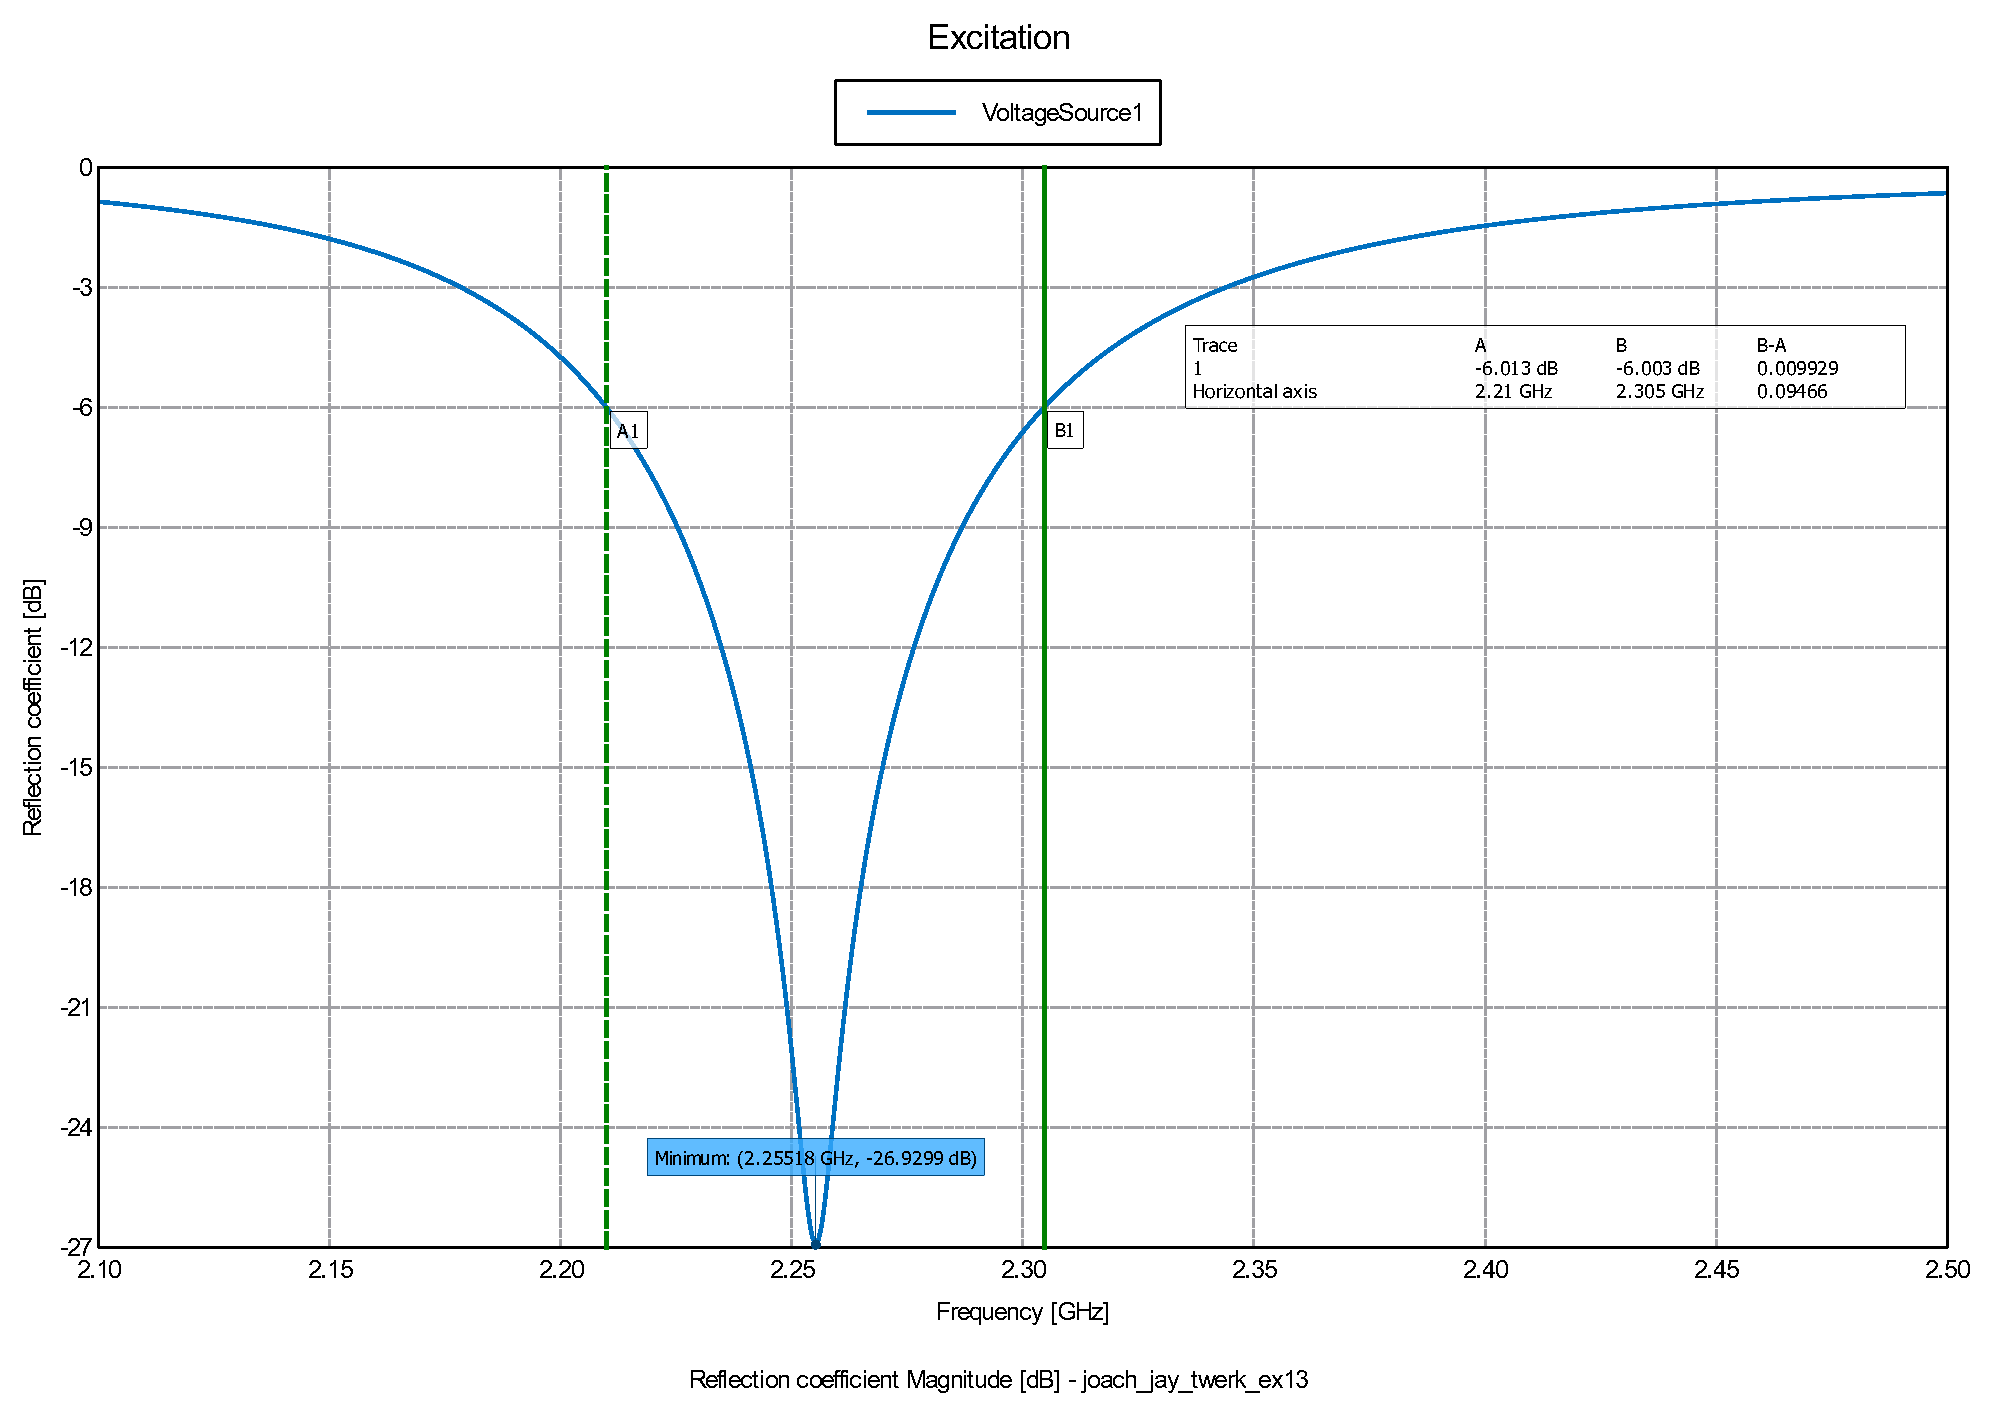
\includegraphics[width=\textwidth]{reflection13_annotation.pdf}
\caption{Coefficient de réflexion en fonction de la fréquence, avec fente de \SI{8}{\milli\meter}}
\label{fig:reflection13_annotation}
\end{figure}

\subsection{Dimensionnement final de l'antenne commandée}
Pour terminer, nous avons alimenté l'antenne par un microstrip inséré dans la fente de l'antenne de la section précédente. A la première itération, ni le coefficient de réflexion, ni la fréquence de résonance ne répondaient au cahier des charges, nous avons donc dû modifier les paramètres de notre antenne de manière à s'approcher le plus possible du résultat demandé.
\begin{figure}[htbp]
\centering
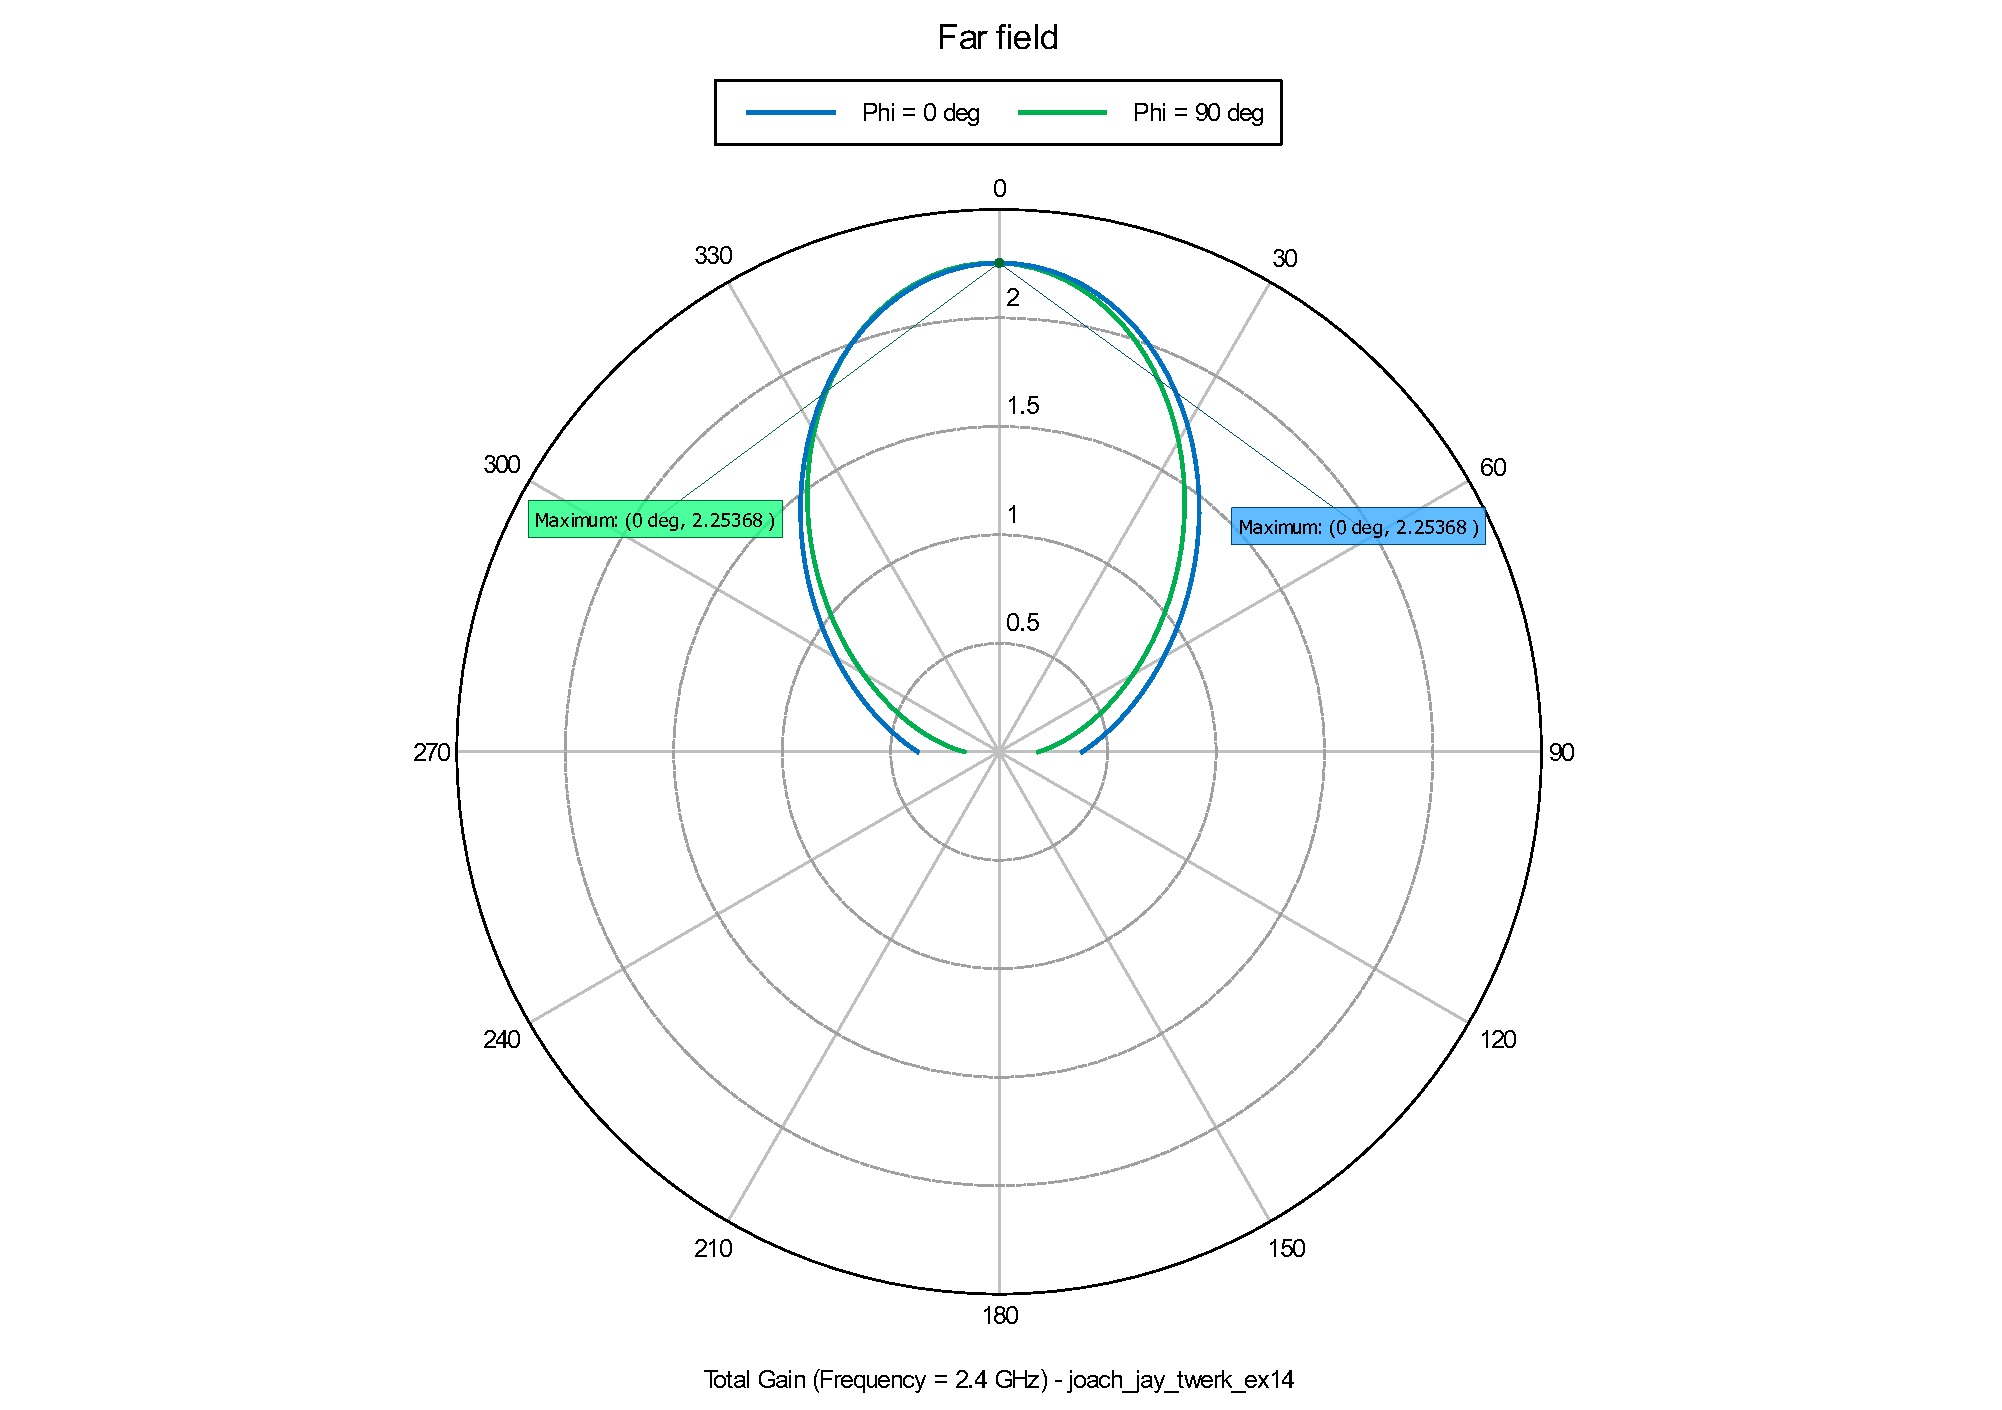
\includegraphics[width=\textwidth]{rayonnement_annotationFinal.pdf}
\caption{Diagramme de rayonnement de notre antenne}
\label{fig:rayonnement_annotationFinal}
\end{figure}
Comme on peut le voir sur la figure \ref{fig:rayonnement_annotationFinal}, le gain maximum de notre meilleure itération vaut \SI{2.25}. La directivité quant à elle vaut \SI{4.02}. Le rendement de l'antenne est défini comme le rapport des deux et vaut \SI{0.56} (le rendement est indépendant de $\theta$ et $\phi$). Le coefficient de réflexion est quand à lui donné à la figure \ref{fig:reflection_annotationFinal}.
\begin{figure}[htbp]
\centering
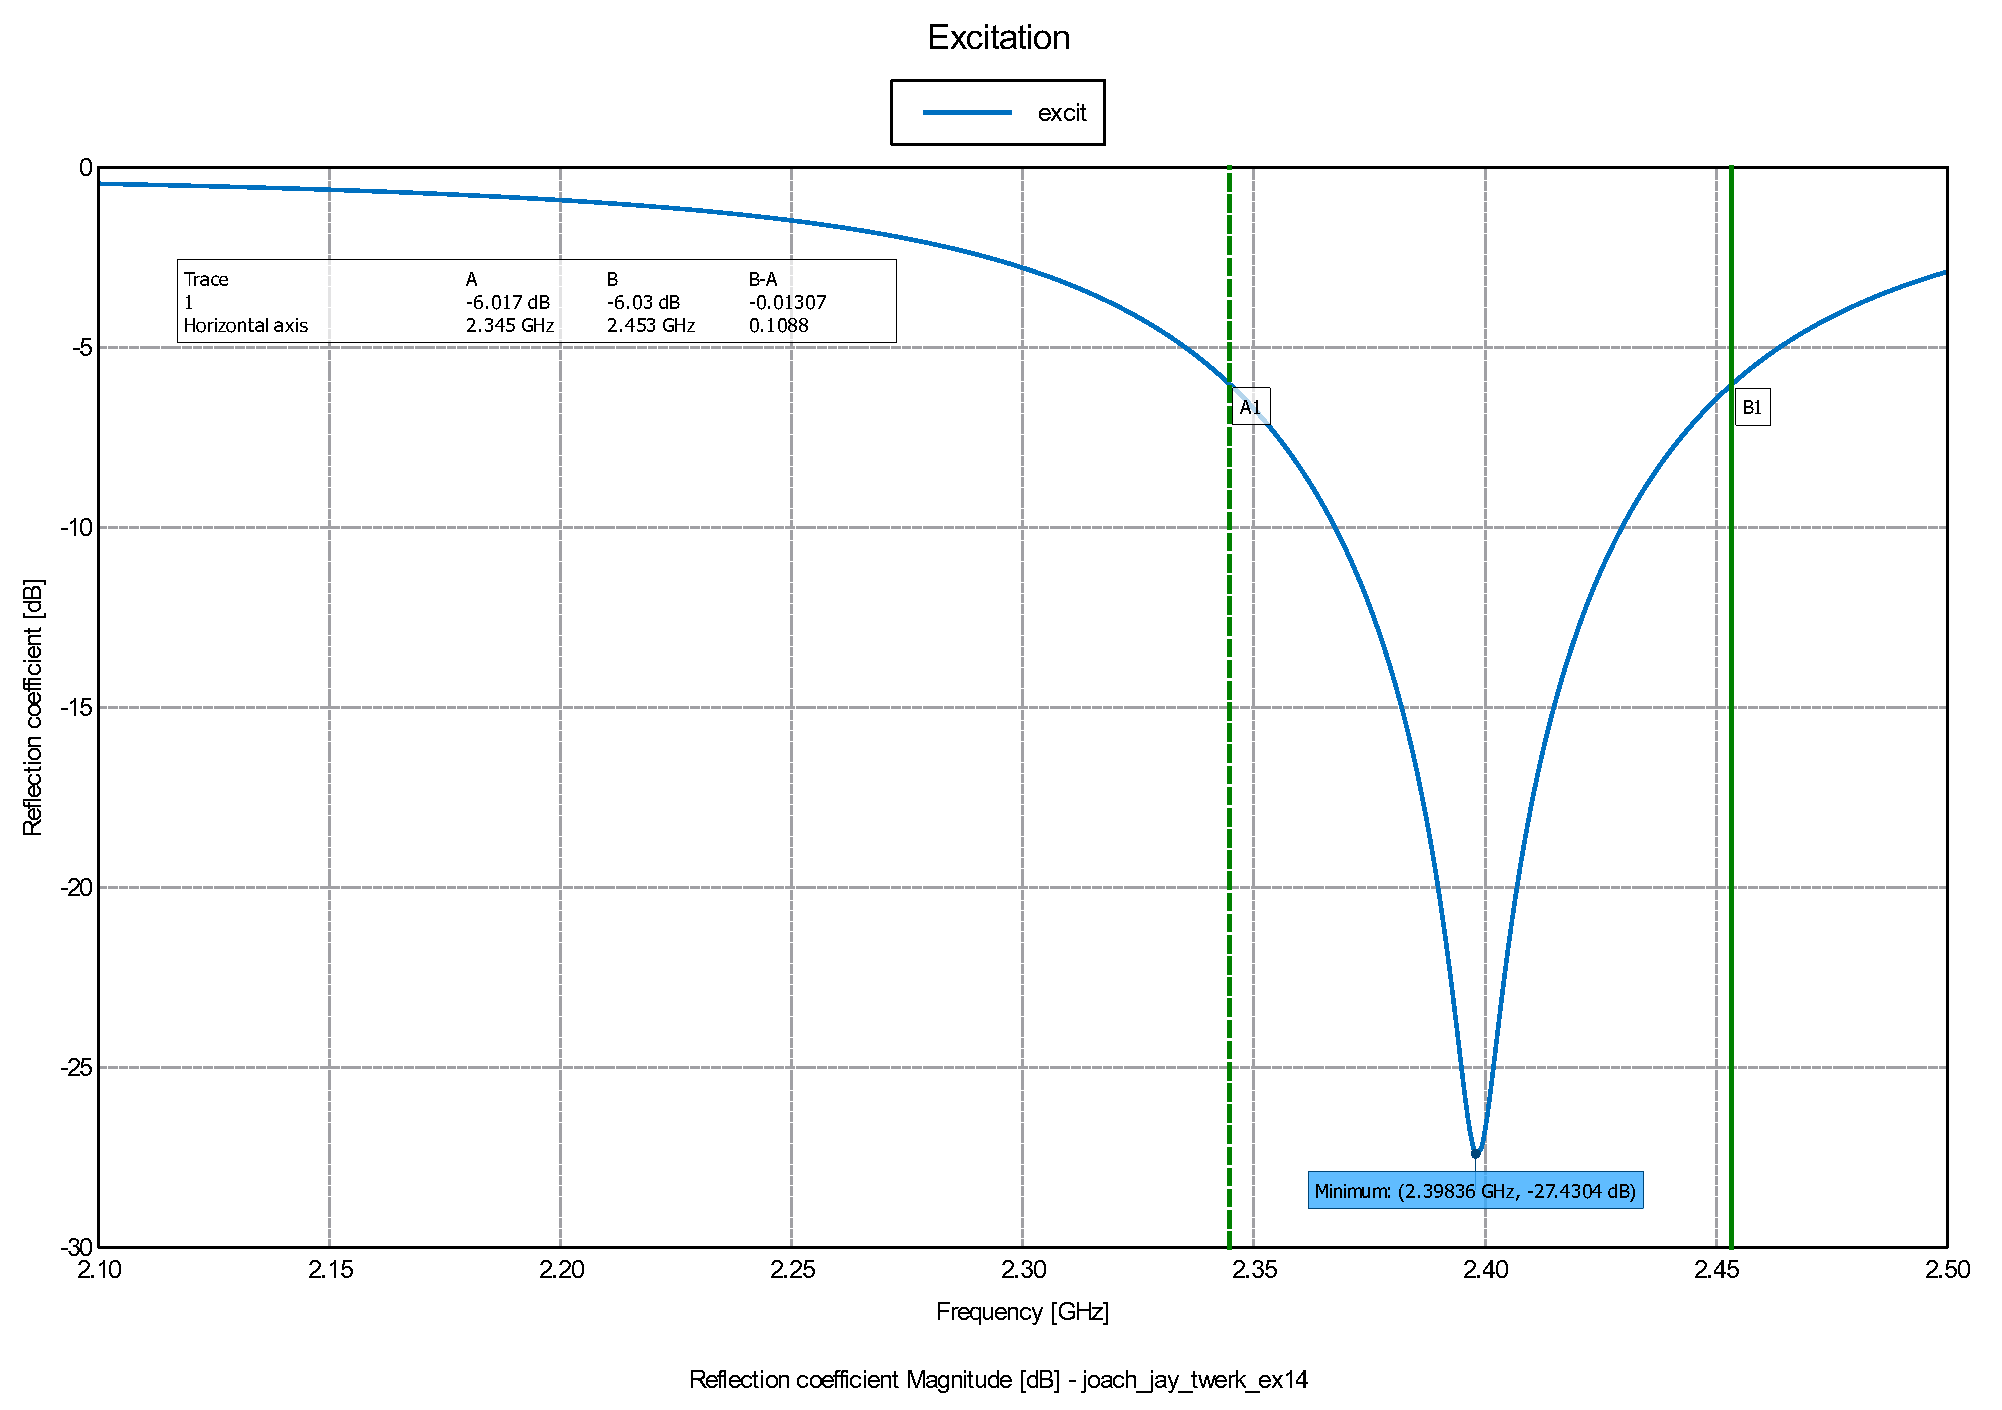
\includegraphics[width=\textwidth]{reflection_annotationFinal.pdf}
\caption{Coefficient de réflexion de notre antenne en fonction de la fréquence}
\label{fig:reflection_annotationFinal}
\end{figure}

Pour conclure ce premier laboratoire, nous avons calculé la puissance reçue par notre antenne si une antenne identique émet \SI{1}{\milli\watt} à un mètre de distance. Pour cela, nous avons utilisé la formule de Friis (\ref{eqn:Friis}). Le bilan de liaison donne une puissance à la réception de \SI{0.5}{\micro\watt}.

\begin{equation}
P_{RX}(d) = P_{TX}G_{TX}(\theta_{TX},\phi_{TX})G_{RX}(\theta_{RX},\phi_{RX})\left(\frac{\lambda}{4\pi d}\right)^2
\label{eqn:Friis}
\end{equation}


%Bonjour, bien dormi?
%Aussi étonnant que ça puisse paraître, \includegraphics[width = x \textwidth]{file.pdf} veut dire que tu redimensionne la figure pour qu'elle soit aussi large que x fois la largeur du texte à cet endroit. A toi d'ajuster à ta guise. Mais ne t'en fais pas, je passerai quand même derrière pour râler malgré tout. U b saf mah nig
